\documentclass[useAMS,usenatbib]{mn2e}

\usepackage{epsfig}
\usepackage{epstopdf}
\usepackage{lscape} % Allows landscape environment to be used

\def\gtrsim{\mathrel{\hbox{\rlap{\hbox{\lower4pt\hbox{$\sim$}}}\hbox{$>$}}}}


\title[Interstellar Plasma Scattering]{
**Pulsar scintillations from corrugated reconnection sheets in the ISM**
!!Origin of Interstellar Scintillations!! 
}
\author[Pen and Levin]{Ue-Li
  Pen,$^{1}$\thanks{E-mail:\ pen@cita.utoronto.ca}
Yuri Levin,$^2$\thanks{E-mail:\ yuri.levin@monash.edu}
}
\begin{document}


\date{\today}

\pagerange{\pageref{firstpage}--\pageref{lastpage}} 
\pubyear{2012}

\maketitle
\label{firstpage}
\begin{abstract}

We show that surface waves along !!aligned!! interstellar current sheets **closely aligned
with the line of sight**
lead to pulsar scintillation properties consistent with those
observed.  !!It!! **By contrast with previously considered scintillation drivers, our mechanism** !!resolves several ISM challenges to explain!! **naturally
produces** the length
!!scales!! and density scales **of the ISM scattering lenses that are required to explain the magnitude and
dynamical spectrum of the scintillations**.  In !!this!! **our** picture, the **parts of warm ionized** interstellar
medium **that are responsible for the scintillations** !!is!! **are relatively** quiescent, with scintillation and scattering resulting from
weak waves propagating along magnetic domain boundary current sheets,
which are **both** expected from helicity conservation **and have been observed in numerical
simulations**.  !!This!! **The** model
quantitatively predicts the spacing and amplitudes of inverted
parabolic arcs **seen in Fourier-transformed dynamical spectra of strongly scintillating pulsars**.  !!We present results for 1-D simulations.!! THE LAST SENTENCE IS NOT INFORMATIVE; IT SHOULD EITHER
BE DROPPED OR CONTINUED AS "..AND FIND THAT"
**We suggest that** Multi-Frequency, multi-epoch VLBI observations can quantitatively test
this picture.  If successful, in addition to mapping the ISM, this
opens the door to precise nanoarcsecond pulsar astrometry, distance
measurements, and emission studies using these 100AU interferometers
in the sky. THE LATEST STATEMENT IS CURRENTLY NOT BACKED UP BY ANYTHING IN THE PAPER.

\end{abstract}
\begin{keywords}
Interstellar Medium, reconnection, extreme scattering events ARE WE EVEN MENTIONING THE 
EXTREME SCATTERING EVENTS?
\end{keywords}

\newcommand{\be}{\begin{eqnarray}}
\newcommand{\ee}{\end{eqnarray}}
\newcommand{\beq}{\begin{equation}}
\newcommand{\eeq}{\end{equation}}

\section{Introduction: **observations and theoretical challenges**}

The structure of the I THINK WE SHOULD FOCUS THE READERS ATTENTION ON WHICH PART OF THE
INTERSTELLAR MEDIUM WE ARE CONSIDERING AND ON WHAT SCALES interstellar medium has remained enigmatic. Five
decades of pulsar scintillation observations \cite{1968Natur.218..920S}
have resulted in problematic physical requirements I THINK WE NEED TO GIVE SEVERAL MORE CITATIONS
FOR THE FIVE DECADES.  Current
observations have demonstrated that much of the scattering is
dominated by a small number of very localized lensing
screens \citep{2010ApJ...708..232B} along the line of sight WHAT IS THE STRONGEST EVIDENCE 
FOR THIS? I THOUGHT THIS WAS PARABOLIC ARCS. IF SO WE SHOULD SAY SMTHG LIKE
**Major observational progress of the ISM scintillations has been achieved through the
Stinebring et al.~(2001) detection of parabolic structures in the Fourier-tranformed dynamical
spectra of strongly scintillating pulsars. These parabolic structures imply that for these pulsars
the  radio-wave scattering
occures mostly within one or several thin screens (Walker et al.~2004, Cordes et al.~2006, 
Walker et al.~2008). Moreover, the multiple "inverted parabolae" (Hill \& Stinebring 2005, 2007)
show that the scattering inside the screen is strongly inhomogeneous but instead occures in localized
clumps. The latter was recently confirmed by Brisken et al.~(2010) who have obtained the VLBI scattering
 image PSR... . They have found that not only the scattering image was clumpy but that the clumps lined 
 up along a thin line.** (SHOULD WE ALSO MENTION THE SECOND CLUMP?)  !! Within
the lensing screen, the scattering is in turn dominated by spatially
localized structures.!!  **All of these observational facts
 present a major challenge for theoretical interpretation
where the scattering is caused by a turbulent cascade. In particular, (1) the origin of
the screens is unexplained, and (2) the strongly non-gaussian scattering on the  requires AU-size regions of which are over-pressurized by factors of $\sim 10^3$ relative to the ambient warm ISM (REFERENCE?); no
conventional physical mechanism has been proposed for how such regions may be formed.

Radio-wave scattering by non-turbulent large-scale refractive structures has been previously
considered by Romani, Blandford, \& Cordes (1987), mostly in the context of the so-called
extreme-scattering events observed by Fiedler et al. Recently, Goldreich and Sridhar (2006) proposed that the image of the SgrA* radio-source is 
strongly scattered by several reconnection sheets that are closely aligned with the line of sight to
SgrA*.
In this paper, we develop further the Goldreich \& Sridhar's (2006) idea [see also Pen \& King 2011] 
and apply it to construct a quantitative
picture of pulsar scintillations. Namely, we consider a scenario where
the pulsar radio-wave scattering occurs due to several {\it weakly corrugated} 
reconnection sheets that are
closely aligned with the line of sight to the pulsar.  We show that this scenario provides
compelling explanations for previously unexplained features of the scintillations: 
(1)  the "scattering screens" are simply effective descriptions of such sheets; their location is marked 
approximately
by the sheets' intersections with the line of sight, (2) "the scattering clumps" correspond to 
those parts of sheet folds where the sheet is parallel 
to
the line of sight; the strength of the scattering follows a strongly non-Gaussian distribution, even though
the corrugation itself is assumed to be a realization of a Gaussian distribution, and (3) the
strong non-isotropy of the Brisken et al. 2010 image is a consequence of the sheet's inclination, 
with the clump locations aligned along the sheet's line of nodes. The plan of the paper is
as follows: in the next section we briefly describe the origin of the
reconnection sheets, in section 3  we derive the model for the fold statistics,
in section 4 we derive the lensing by the corrugated sheet, and in section 5 we compute the
Fourier-transformed dynamical spectrum and demonstrate the parabolic structures. In section 6 we conclude.**  !!This is difficult to understand with random diffractive
processes in an extended turbulent medium.!!

UE-LI, I WOULD PROPOSE TO MAKE THE NEXT 3 SECTIONS INTO 3 SUBSECTIONS OF A LARGER SECTION
CALLED "ASTROPHYSICAL PICTURE".  I'D ALSO PUT  THE "TWO REGIMES OF LENSING" SUBSECTION
LAST SINCE NOW IT SORT OF COMES OUT OF NOWHERE.
\section{Two Regimes of Lensing: Diffractive vs Refractive}

Two regimes to generate pulsar scintillation have been considered. In
the diffractive !!picture!! **regime**, the scattering/lensing angle is determined by
the size of structure in the medium, compared to the wavelength
$\lambda$: $\theta=2\pi\lambda k$. WE HAVE TO DEFINE $k$. IT IS THE CHARECTERISTIC WAVEVECTOR 
OF A SCATTERING STRUCTURE PERPENDICULAR TO THE LINE OF SIGHT, RIGHT?  The amplitude of !!each!! scattered
!!structure!! **image** IN THE PREVIOUS SENTENCE WE USED "STRUCTURE" AS IN PERTURBATION IN THE ISM,
BUT HERE WE USE STRUCTURE AS IN PERTURBATION IN THE SCATTERING IMAGE. FORM THE POINT OF VIEW
OF THE LANGUAGE, THESE ARE DISTINCT is determined by the !!depth!! **amplitude** of the **wavefront** modulation **caused by the scattering structure**.  To explain
the observed angles in the range $1-100$ mas at wavelength $\sim 1$m,
requires structures in the ISM on scales of order $10^{6-8}$m. This
imposes unexpected properties on the **warm ionised** interstellar medium SHOULD WE GIVE IT
AN ABBREVIATION ONCE AND FOR ALL, WISM?, since it is
much smaller than the coloumb mean free path of free electrons !!in the
interstellar medium!!.  In !!such mechanism!! **this scenario**, the angular image of a
pulsar, and therefore its dynamic spectrum, are superpositions of many CAN WE ESTIMATE HOW MANY?
IS THIS NOT JUST (AU/10$^8$M)~10$^3$ FOR A 1-D SCATTERING IMAGE?
weak structures, and are expected to be roughly gaussian.  The
parabolically structured 2-D power spectrum of the dynamic spectrum,
and the VLBI image of the scattering disk, are inconsistent with such
a picture, at least for the long-lag (ms) structures.

A second mechanism is due to refractive lensing.  In this scenario,
the bending angle is determined by Snell's law, i.e. the change in
refractive index and the angles of incidence.  The flux of the images
is determined by the size of the lens over the impact parameter.  This
picture is also challenging to implement, since the observed
scattering angles would na\"ively require changes in free electron
density of $\sim 10^3$ IS THERE A VERY QUICK ESTIMATE TO
SHOW THAT IT'S TRUE?, which are difficult to understand or confine.

\cite{2006ApJ...640L.159G} showed that refractive lensing results in
scintillation similar to the diffractive picture.  In this refractive
lensing, localized refractive images act like a multiple slit
interferometer. The beating of these images results in the rapid
frequency and time variability, and has scalings WHAT EXACTLY SCALINGS? I THINK WE
HAVE TO BE MORE SPECIFIC very similar to the
purely diffractive picture. 

!!The discovery of parabolic arcs\citep{2001ApJ...549L..97S} and
inverted arclets has required the existence of localized refractive
lenses.  Direct VLBI imaging of the scattering
screen\citep{2010ApJ...708..232B} demonstrate the presence of
discrete isolated lenses, i.e. scattering points, which are all in a
single thin sheet. This leads to physical challenges of confining
these lenses. Various solutions have been
proposed\citep{2007ASPC..365..299W,2012MNRAS.421L.132P,2006ApJ...640L.159G}.

In this paper, we expand the picture of current sheets, and consider
perturbations.!!


\section{Astrophysical Picture}

The interstellar medium is stirred on scales of parsecs by various
energetic processes, including supernovae, ionization fronts, spiral
density waves, and other phenomena.  These processes are generally
short lived, and **we conjecture*** after the stirring, the warm medium relaxes to an
**near-**equilibrium configuration **on small (several AU) scale. Current numerical
simulations of the supernova-driven turbulence in the warm ISM of the Galaxy (e.g., Hill et al.~2011)
do not have the resolution to tell how realistic this assumption is.**  In the presence of helicity, the
equilibrium magnetic fields are configured as interlaced twisted tori,
which are long lived \citep{2004Natur.431..819B}.  **It has been shown by Gruzinov (2009)
that a "generic magnetic equilibrium of an ideally conducting fluid contains a volume-filling set of singular current layers." In this picture,** the magnetic fields
are locally almost parallel, with discontinuous interface regions, a
bit like magnetic domains in a ferromagnet. **Singular current sheets have also been seen in the
simulations of Schekochihin et al.~(2004; ApJ, 612, 276 -  YL.)**

At the boundary between between magnetic field configurations, current
sheets maintain the discontinuities.  These current sheets have been
proposed to dominate the scattering of radio
sources \citep{2006ApJ...640L.159G}.

\section{Surface Dynamics}

The current sheet is physically thin, $< \sim $ AU (IS THIS FROM GOLDREICH \& SRIDHAR?
IS THERE A SIMPLE ARGUMENT FOR THE READER?).  On each side the
magnetic field points in a different direction.  The change in alvenic
properties gives rise to surface
wave \citep{1991SoPh..133..263J, 2009GApFD.103...89J}, **whose amplitude
decays exponentially with the distance to the current sheet and** which are
**mathematically** analogous to deep water ocean waves.  The restoring force is **due to** the
difference in magnetic field component projected along the wave
vector.  Like ocean waves, these waves penetrate about a wavelength
into each side.  We will be considering wavelengths of thousands of
AU WHY?, so the **thickness of the** current sheet itself is neglible as far as the dynamics of
the waves are concerned.  Seen in projection along the aligned sheet,
the projected wavelengths will be $\sim $ AU IS THIS BECAUSE THE ALIGNMENT ANGLE IS
$\sim 0.001$?  THIS IS THE FIRST TIME THAT THE MAGNITUDE OF THE ALIGNMENT ANGLE
IS DISCUSSED; MAY NEED A BIT MORE EXPLANATION.  The displacements are
transverse to the wave vector, and perpendicular to the sheet.  While
alvenic in nature, the surface modes possess only one polarization,
unlike bulk waves.  These waves resemble a flag blowing in the wind.
Disturbances travelling along the sheet are decoupled from bulk waves.
Being confined to a sheet, the amplitude away from a source drops as
$\propto 1/r$ instead of the normal inverse square law.  A amplitude
of order $\alpha \lambda$, HERE $\lambda$ IS THE WAVENENGTH OF THE SURFACE WAVE BUT
IT WAS PREVIOUSLY USED FOR THAT OF RADIO WAVES or about $10^{-3}$ of the wavelength is
sufficient to cause the sheet to appear folded in projection.

\section{Fold Statistics}

Alven waves dissipate on scales shorter than the proton mean free
path WHICH IS WHAT IN THE WISM? REFERENCE?.  We thus model the waves as a displacement function $\zeta(x)$
which is a Gaussian random field with a correlation function that is a
Gaussian, $\xi(r)=\langle \zeta(x)
\zeta(x+r)\rangle=A^2\exp(-r^2/2/\sigma^2)$, where **$A$ is the mean amplitude
of the displacement and** $\sigma$ is the **surface-wave**
dissipation scale.  Figure \ref{fig:sheet} shows a realization of a
sheet with a random fluctuations.

\begin{figure}
\centerline{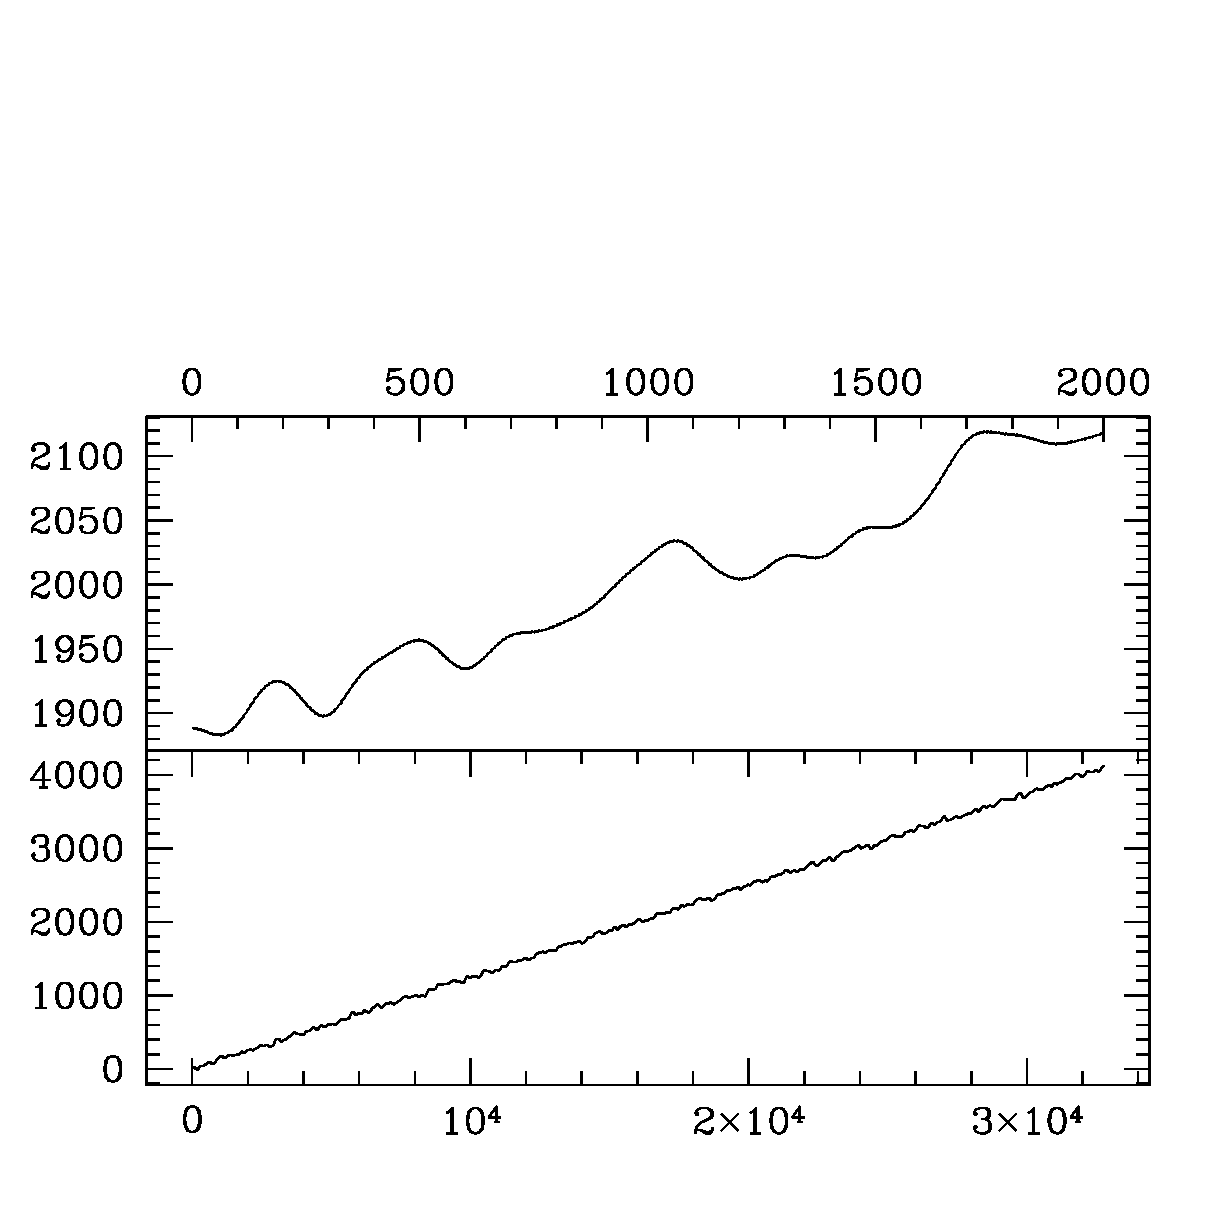
\epsfig{file=sheet.eps,width=3in}}
\caption{Sheet with transverse perturbations.  The upper panel shows
  an zoomed version of a short section.}
\label{fig:sheet}
\end{figure}

**The current sheet has a reduced magnetic pressure and thus has a refractive index different
from the ambient ISM. For simplicity, we assume here that the sheet has constant thickness, and
consider its optical depth as is relevant for refractive lensing.**
In projection **along the line of sight**, the !!surface!! **column** density of the !!current!! sheet 
results in a highly non-Gaussian
distribution. Figure \ref{fig:rho} shows the **column** density distribution in a
simulation.  Folds occur when the gradient of the displacement is
equal to minus 1 NO, IT IS $-\alpha$ WHERE ALPHA IS THE INCLINATION ANGLE.  The correlation function of the gradients is the
second derivative of the displacements.  The number of crossings of -1
depends on the variance of the gradient field.  The density of the
folded sheet is proportionate to the length of gradient spent in the
vicinity of -1, which is turn is proportionate to the reciprocal of
the derivative of the gradient.  This second derivative is also a
Gaussian random field.  The second derivative is uncorrelated with the
first derivative.  The one point PDF of the reciprocal of a Gaussian
variable is
\beq
P(\rho)=\frac{\exp(-\frac{1}{2 \rho^2})}{\sqrt{2\pi}\rho^2}.
\eeq
UE-LI, I GET A DIFFERENT ANSWER. I DON'T HAVE THE FULL EXPRESSION, BUT 
ASYMPTOTICALLY THE HIGH-END TAIL IS CLEAR. LET $\theta$ BE THE ANGLE BETWEEN THE 
SCREEN AND THE LINE OF SIGHT.  THEN THE OPTICAL DEPTH IS $\rho\propto1/\theta$ FOR
$\theta\ll 1$ AND $P_{\rm screen}(\rho)\propto 1/\rho^2$, WHERE $P_{screen}(\rho)$ IS THE PROBABILITY OF A PIECE OF SCREEN TO HAVE THE OPTICAL DEPTH OF $\rho$. HOWEVER, WE ARE INTERESTED
IN THE PROBABILITY DENSITY WITH RESPECT TO THE IMPACT PARAMETER, AND NOT WITH RESPECT TO
THE LOCATION ON THE SCREEN. FOR NEARLY ALIGNED SCREENS, THIS IS NOT THE SAME THING.
IN PARTICULAR, PART OF THE SCREEN WITH LOW $\theta$ OCCUPIES LESS OF THE IMPACT-PARAMETER
SPACE THAN THE PART OF THE SCREEN WITH HIGH $\theta$. THUS, 
\begin{equation}
P_{\rm impact parameter}(\rho)\propto 1/\rho^3
\end{equation}
STILL VERY NON-GAUSSIAN, BUT WITH THE SOFTER POWER-LAW. 
probability of a piece of screen  is a highly non-Gaussian distribution, and resembles a Lorenzian,
with divergent moments SO NOT THE LORENTZIAN, BUT SOFTER.  The very
high tails are 
cut off by higher order derivatives of the correlation function.

\begin{figure}
\centerline{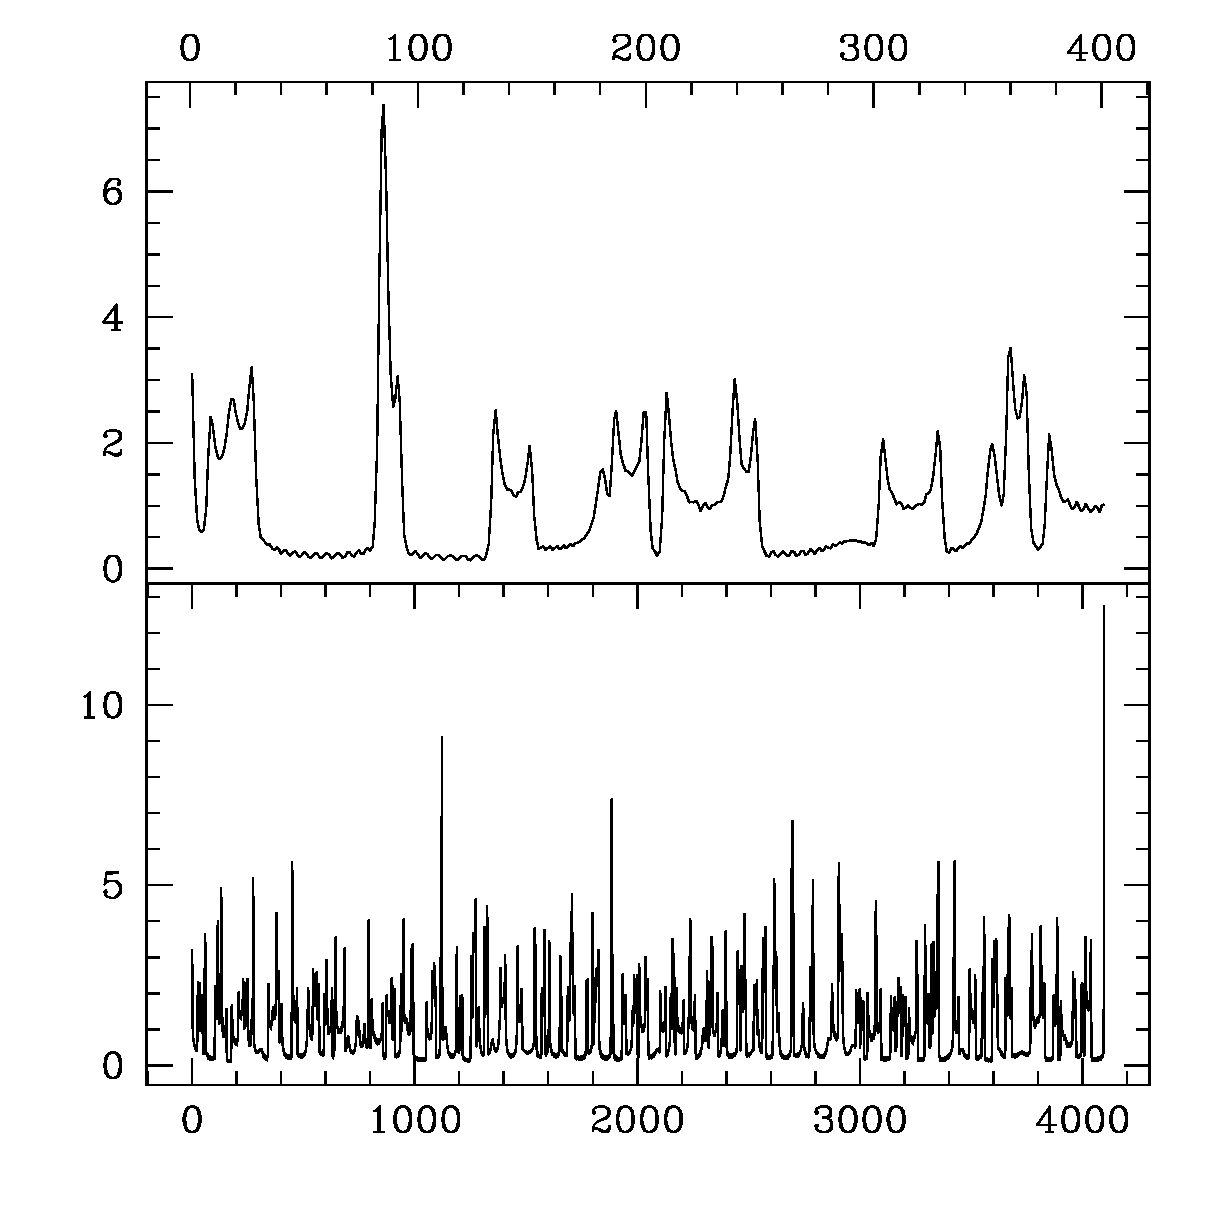
\epsfig{file=rho.eps,width=3in}}
\caption{projected density.  The upper panel is a zoom of the central
  portion of the lower panel. Each time the sheet folds in projection,
we see a caustic structure in density.}
\label{fig:rho}
\end{figure}

!!These high density caustics!! **The regions near the locations where the screen is parallel
to the line-of-sight, which the call the caustics,** give rise to !!refractive lensing processes
which resemble!! **the localized clumps in the pulsar's scattering image, which
produce** the inverted parabolic arcs in pulsar secondary
spectra.

\section{Lensing}

The lensing of this density sheet can be computed in analogy to 
 \cite{2012MNRAS.421L.132P}.

\begin{figure}
\centerline{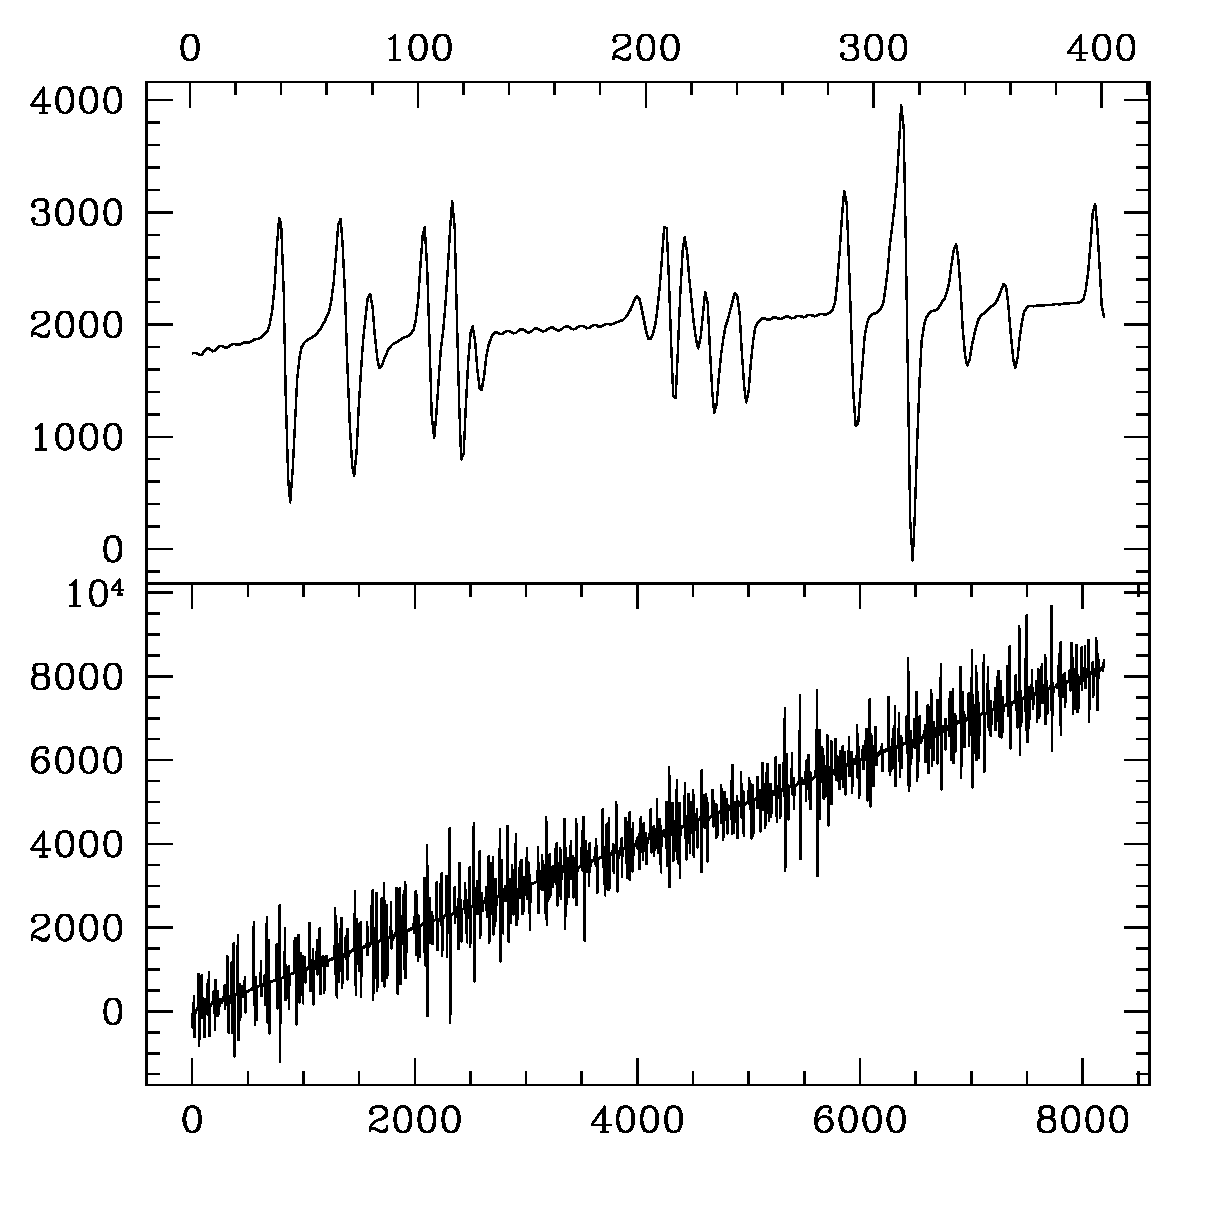
\epsfig{file=dt.eps,width=3in}}
\caption{deflection angle mapping. The horizontal axis is angle on the
sky, and the vertical axis is the intersection of this light ray on
the source plane.  Whenever multiple different directions on the sky
intersect on the same position in the source plane, multiple images
are formed, which form a coherent interference pattern.}
\label{fig:dt}
\end{figure}

Given the projected **column** density distribution in Figure \ref{fig:rho}, **and assuming that
the sheet has a fixed optical depth along its normal**, we
can compute the mapping of apparent angle on the sky to position in the
source (pulsar) plane.  The caustics in the projected density
distribution lead to large angle deflections, and multiple imagine,
whenever the sheets are aligned closer than the amplitude of the
perturbations.  This explains why only a small fraction of (edge-on) current
sheets contribute to scintillation.

\section{Simulated Dynamic Spectra}

With the density field, we can solve the lens equations to simulate
dynamic spectra.  By adding the voltages on each image  with their
appropriate amplitude and phases, we simulate the dynamic spectrum,
shown in figure \ref{fig:ds}.
DO YOU WANT TO SAY A FEW WORDS ABOUT THE PROCEDURE THAT YOU USED
TO GENERATE THE DYNAMICAL SPECTRA? IF YOU FOLLOWED SOMEBODY'S
METHOD, DO YOU WANT TO REFER TO THIS PAPER?
\begin{figure}
\centerline{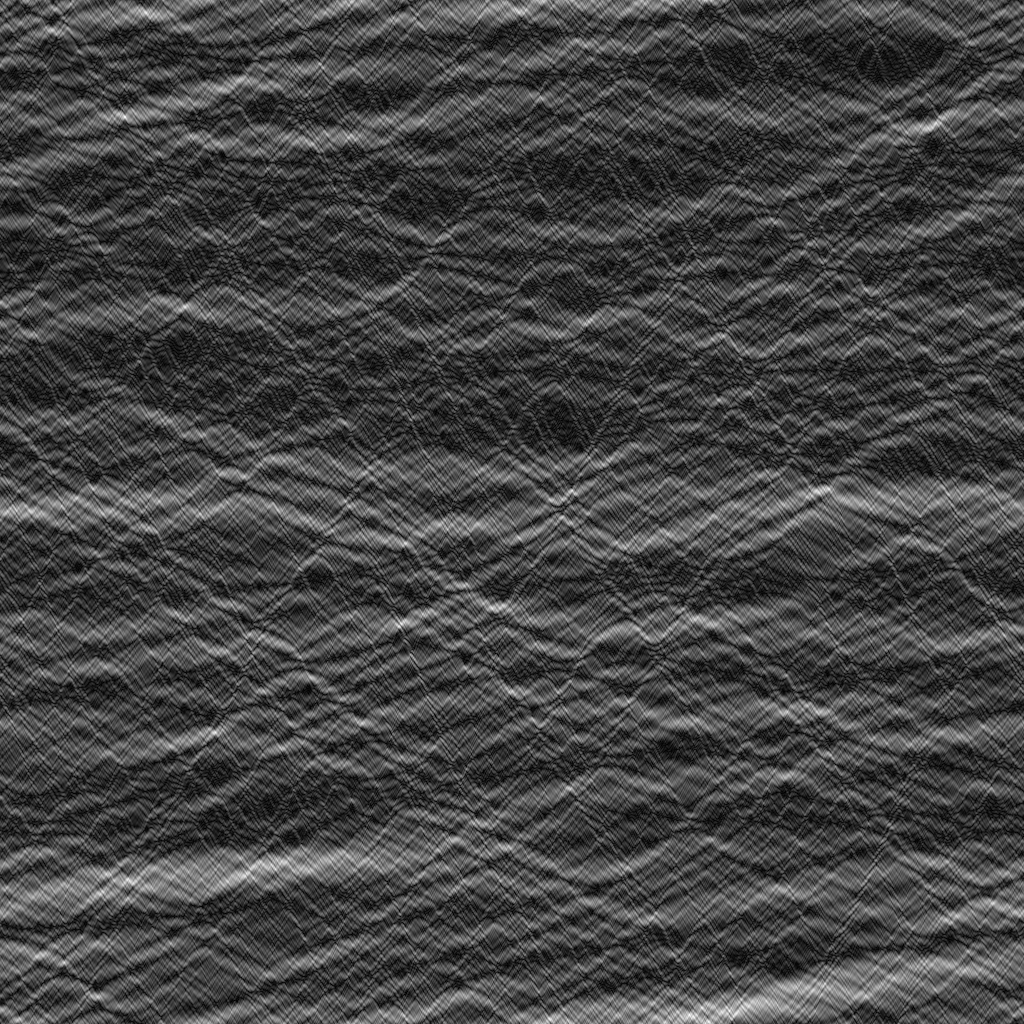
\includegraphics[width=3.5in]{rspect.jpg}}
\caption{dynamic pulsar spectrum.  Horizontal axis is time, vertical
  axis is frequency.  We reproduce the characteristic criss-cross
  pattern observed in real scintillation spectra.}
\label{fig:ds}
\end{figure}

A 2-D fourier transform maps this dynamic spectrum into a secondary
spectrum, shown in figure \ref{fig:ss}.

\begin{figure}
\centerline{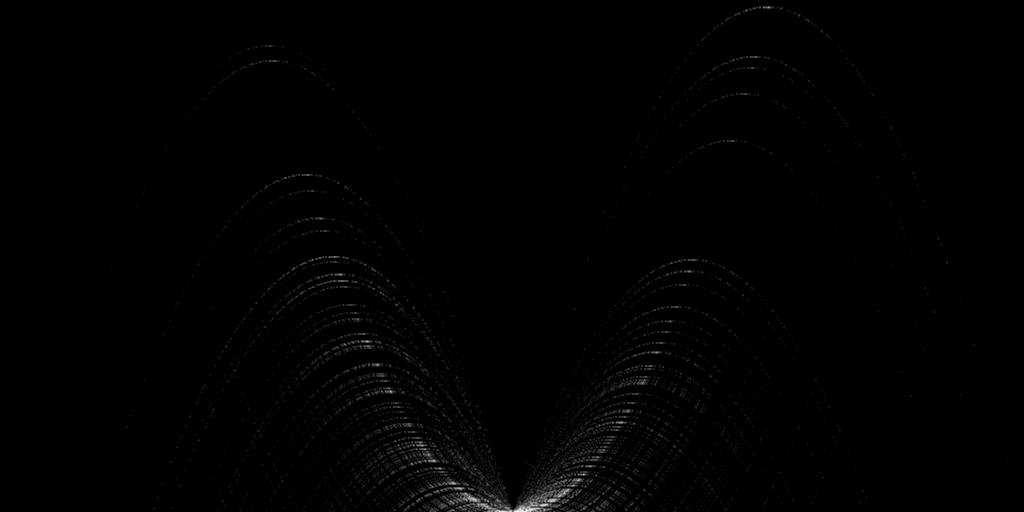
\includegraphics[width=3.5in]{sspect.jpg}}
\caption{secondary pulsar spectrum.  The inverted parabolic arcs arise
naturally in this model.}
\label{fig:ss}
\end{figure}

We find that the interference of these discrete, co-linear images
forms the inverted parabolic arcs, **qualitatively similar to those** that are observed **in
Stinebring et al.~(2001) and Hill et al.~(2005), (2007).

\section{Discussion}

We can estimate the length scales involved **in making the current sheet that
would produce the observed scintillation pattern**.  This theory requires as
input a current sheet thickness, inclination angle, curvature,
amplitude of waves, and dissipation scale.

The thickness of the sheets is determined by the magnification of
images: the flux is roughly the thickness divided by the impact
parameter WHY? NOT OBVIOUS TO READERS LIKE ME.  
It suggests a typical tickness of $h\sim 0.1$ AU WE SHOULD QUOTE SOME
OBSERVATIONAL PAPER WHERE THESE MAGNIFICTIONS ARE MEASURED.  A wave
of projected wavelength $\alpha \lambda$ enhances projected densities
by a factor $w=\sqrt{h \alpha \lambda}$ THIS FACTOR SHOULD BE 
DIMENSIONLESS. I GET $\sqrt{\alpha\lambda/h}$  The projected wavelengths
are known to be of order $\sim 10$ AU, so $w \sim 10$.  The largest
deflection angles are $\gamma \sim 0.1$ mas, which requires a
projected electron density change $\delta n_e/(w\alpha) \sim$ ??.  In an
underdense sheet, the maximal change of density is the density itself.
For the mean interstellar medium densities determined from pulsar
dispersion, we obtain $\alpha \sim 10^{-2}$.  The probability of
seeing a sheet at such an angle is $\sim \alpha^2$ I THINK IT SCALES
$\propto \alpha$, NO? YOU ESSENTIALLY WANT THE NORMAL VECTOR TO
THE SHEET BE WITIN $\alpha$ FROM 90 DEGREES, SO IF YOU ASSUME NORMAL VECTORS
ARE ISOTROPICALLY DISTRIBUTED, YOU GET THE LINEAR SCALING WITH $\alpha$, requiring the
existence of $\sim 1/\alpha^2$ sheets along the line of sight SO I GET 100, NOT
10000.  For
B0834+06, the distance is $\sim 1$ kpc, giving a typical sheet
separation of $s \sim 0.1$ pc.  If we assume the curvature to be
separation (it could be smaller), we find a limiting projection angle
$\alpha_{\rm min} = \sqrt{h/s} \sim 0.002$.  The wave amplitudes must
be $> \alpha \lambda$ in order to form projected caustics.  This is a
small amplitude, which rules out large amplitude universal turbulence.
The latter would deform the sheet too much.  In a Kolmogorov spectrum,
the energy power spectrum scales as $k^{-5/3}$.  Scaling from the
alven damping scale to the fresnel scale, this results in density
fluctuations $< 10^{-4}$.  This is insufficient to create
scintillation in pulsar fluxes.

These estimates are qualitative.  One expects current sheets to come
in a range of sizes, curvature and perturbation amplitude.  The
thickness might also vary, unless due to global resistivity.
% 1 kpc = 3e19m
% fresnel scale = 5e9m, 2e-10 radians, 0.04 mas
% for n_e = 0.03, T=10,000K MFP=1/(n \sigma)
% sigma=(1e-7 log lambda)^2 cm^2 = 1e-12 cm^2, mfp=3e13 cm = 3e11m
% 1 AU = 1.5e11 m

UE-LI, I THINK ONE OF THE ATTRACTIVE FEATURES OF OUR MECHANISM IS THAT IT EXPLAINS VERY NATURALLY THE 1-D IMAGE OF BRISKEN ET AL. IMHO IT WOULD BE VERY GOOD IF YOU SHOWED
THE 2-D SCATTERING IMAGE AND DEMOSTRATED THAT THE SCATTERING CLUMPS ARRANGE ALONG A 
LINE. IT MATTERS NOT THAT THIS RESULT IS PRELIMINARY AND WILL BE INVESTIGATED FURTHER;
AS A PICTURE-SETTER, IT IS VERY IMPORTANT.

\section{Conclusions}

We have presented a quantitative theory of pulsar scintillation
inverse parabolic arcs.  These extend recent ideas of **Goldreich \& Sridhar (2006) and
Pen \& King (2011) about** thin current
sheets as the scattering objects in the ISM**, which naturally explain the large angle 
scattering observed in
pulsars and some extragalactic sources.

This picture could explain all scintillation phenomena with structures
greater than 0.1 AU.  The apparent diffractive structure results from
the interference between refractive images, and no diffractive
scattering is needed.

\section{Acknowledgements}

U-LP thanks NSERC and CAASTRO for support. **YL is supported 
by the Australian Research Counsil Future Fellowship.**


\newcommand{\araa}{ARA\&A}   % Annual Review of Astronomy and Astrophys.
\newcommand{\afz}{Afz}       % Astrofizica
\newcommand{\aj}{AJ}         % Astronomical Journal
\newcommand{\azh}{AZh}       % Astronomicekij Zhurnal
\newcommand{\aaa}{A\&A}      % Astronomy and Astrophysics
\newcommand{\aas}{A\&AS}     % Astronomy and Astrophys. Supplement Series
\newcommand{\aar}{A\&AR}     % Astronomy and Astrophysics Review
\newcommand{\apj}{ApJ}       % Astrophysical Journal
\newcommand{\apjs}{ApJS}     % Astrophysical Journal Supplement Series
\newcommand{\apjl}{ApJ}      % Astrophysical Journal Letters
\newcommand{\apss}{Ap\&SS}   % Astrophysics and Space Science
\newcommand{\baas}{BAAS}     % Bulletin of the American Astron. Society
\newcommand{\jaa}{JA\&A}     % Journal of Astronomy and Astrophysics
\newcommand{\mnras}{MNRAS}   % Monthly Notices of the Roy. Astron. Society
\newcommand{\nat}{Nat}       % Nature
\newcommand{\pasj}{PASJ}     % Publ. of the Astron. Society of Japan
\newcommand{\pasp}{PASP}     % Publ. of the Astron. Society of the Pacific
\newcommand{\paspc}{PASPC}   % Publ. Astron. Soc. Pacific Conf. Proc.
\newcommand{\qjras}{QJRAS}   % Quart. Journal of the Royal Astron. Society
\newcommand{\sci}{Sci}       % Science
\newcommand{\solphys}{Solar Physics}       % 
\newcommand{\sova}{SvA}      % Soviet Astronomy
\newcommand{\aap}{A\&A}


\bibliography{swave}
\bibliographystyle{mn2e}


\label{lastpage}

\end{document}
